% \section{\emph{\sys} Methodology}
\section{\sys Multi-Agent Framework}
\label{sec:methodology}

% This section outlines the \emph{\sys} methodology, which integrates the expertise of human participants and the efficiency of Large Language Model (LLM) agents to convert unstructured software data—such as commit histories and mailing lists—into structured datasets suitable for analysis.
This section presents the \sys multi-agent framework, which creates a virtual Linux community of specialized LLM agents to analyze kernel development. Unlike traditional single-model approaches, \sys employs multiple agents representing different stakeholder perspectives—maintainers, contributors, security experts, and historians—to convert unstructured software data such as commit histories and mailing lists into multi-perspective structured datasets. This approach directly addresses how inner and open-source collaboration will evolve in the FM era.

% The central principle behind \emph{\sys} is to treat LLMs as human participants in a survey-like process. While LLMs can process data more quickly and at lower costs than humans, they are also prone to errors, guesses, and limitations in specific domains, much like human participants~\cite{ji2023survey}. By leveraging traditional survey methodologies designed for humans, we can efficiently conduct LLM-based surveys while maintaining oversight and validation from human experts. Additionally, LLM agents can utilize traditional tools to automate analysis tasks.
The central principle behind \sys is to model the Linux kernel community through specialized agents that embody different stakeholder perspectives. Each agent—Maintainer, Contributor, Security Expert, and Historian—processes kernel artifacts through their unique lens, similar to how real community members have different priorities and concerns~\cite{ji2023survey}. This multi-agent approach reveals how different stakeholders interpret the same changes differently, providing insights into collaboration dynamics. By leveraging agent consensus mechanisms and debate protocols, we can understand not just what changed, but how the community perceives these changes. This cognitive layer serves as a bridge between legacy kernel code and future AIware systems.

\begin{figure}[t]
    \centering
    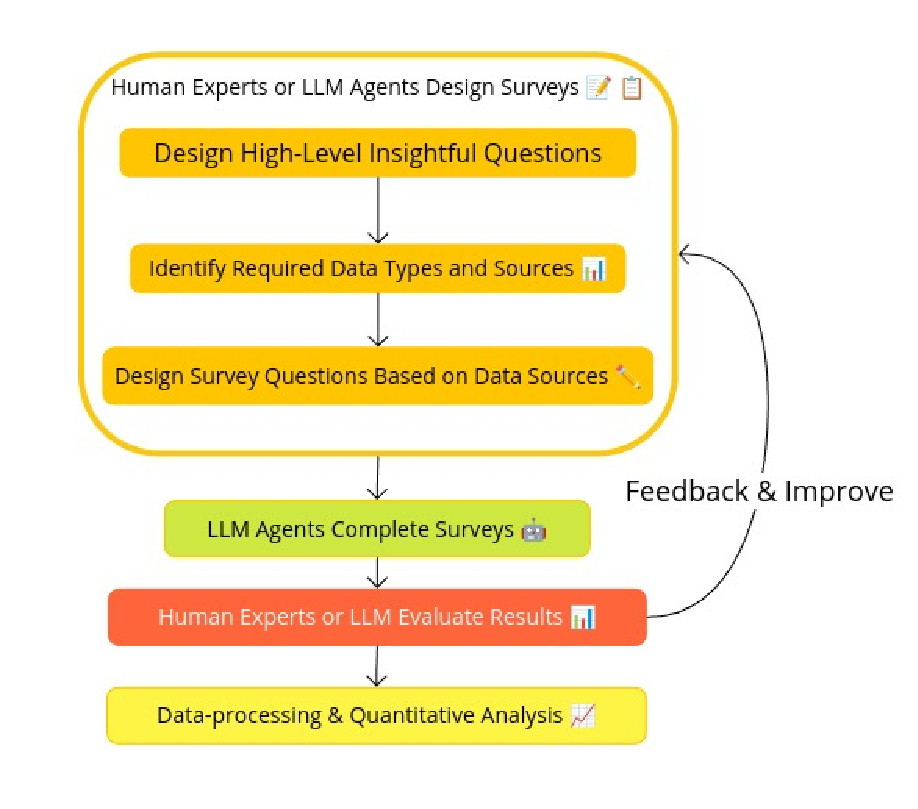
\includegraphics[width=0.5\textwidth]{workflow.pdf}
    \caption{\sys Multi-Agent Workflow}
    \label{fig:workflow}
\end{figure}

\subsection{Workflow}

% The \emph{\sys} process follows a structured workflow, as illustrated in Figure~\ref{fig:workflow}:
The \sys multi-agent process follows a structured workflow, as illustrated in Figure~\ref{fig:workflow}, where specialized agents collaborate to analyze kernel artifacts:

% \begin{enumerate}
%     \item \textbf{Survey Design by Human Experts or LLM Agents}: Experts or LLM agents create tailored questions for each type of unstructured data (e.g., commits, emails) to extract key insights. The survey design is crucial for guiding the LLM in structuring the data effectively and focuses on tasks aligned with the LLM's strengths, such as summarization and yes/no questions. This step should minimizes the usage of open-ended questions that require deep domain expertise.
% 
%     \item \textbf{Survey Completion by LLM Agents}: LLM agents process the unstructured input by answering the survey questions. They organize data into structured formats by tagging relevant information, summarizing key points, and identifying important patterns. This step is fundamental in transforming unstructured data into structured datasets, enabling more straightforward analysis.
% 
%     \item \textbf{Evaluation of Survey Results by Human Experts or LLM Agents}: Human experts with domain-specific knowledge, or additional LLM agents, evaluate a sample of the structured data. This evaluation ensures accuracy and allows for the detection of discrepancies. If the results are unsatisfactory, the process loops back to Step 1, where the survey design is refined.
% 
%     \item \textbf{Data Processing and Quantitative Analysis}: The structured data undergoes further processing to analyze key metrics and patterns. Quantitative analysis is performed to identify trends in development, feature interdependencies, and areas needing improvement in reliability and security. This provides a detailed view of the system's evolution and characteristics.
% 
% \end{enumerate}
\begin{enumerate}
    \item \textbf{Survey Design by Survey-Designer Agent}: A specialized Survey-Designer agent, embodying social science expertise, creates tailored questions for kernel artifacts. This agent ensures questions capture multiple perspectives (stability, features, security, history) and minimizes bias while focusing on extractable insights from commits and emails.

    \item \textbf{Multi-Agent Survey Completion}: Our Community Proxy Agents—Maintainer, Contributor, Security Expert, and Historian—independently analyze each artifact. The Maintainer agent focuses on stability and API compatibility, the Contributor agent on feature velocity, the Security Expert on vulnerability patterns, and the Historian on evolution patterns. Each agent answers the same survey from their unique perspective.

    \item \textbf{Consensus Building via Adjudicator Agent}: An Adjudicator/QA agent collects all agent responses, performs majority voting, calculates inter-agent agreement (Cohen's kappa), and flags low-consensus items for human review. This reveals where stakeholder perspectives diverge—key insights for understanding collaboration evolution in the FM era.

    \item \textbf{Legacy Integration via Data-Loader Agent}: A Data-Loader agent transforms the multi-perspective structured data into modern formats (SQL, GraphQL), creating a cognitive bridge between legacy kernel code and future AIware systems. This enables AI tools to query 30+ years of kernel history without modifying the codebase.

\end{enumerate}

% This process employs an iterative design, allowing surveys to be refined based on analysis results, thereby creating a feedback loop that enhances data structuring and interpretation. By leveraging both LLMs and human oversight, the \emph{\sys} methodology efficiently handles large volumes of unstructured software data. At each step, human experts can interactively contribute, or LLM agents can automate the process.
This multi-agent process reveals collaboration patterns impossible to detect with single models. When agents disagree, it signals areas where real maintainers and contributors likely have different priorities—insights crucial for understanding how OSS collaboration evolves. The framework demonstrates that future kernel development will be AI-augmented rather than AI-replaced, with multi-agent systems serving as cognitive enhancers for human developers. By providing structured access to legacy code through modern interfaces, \sys shows how AIware can integrate with existing systems without disruptive rewrites.

\subsection{Multi-Agent Architecture}

Our multi-agent framework consists of specialized agents that mirror the Linux kernel community:

\textbf{Survey-Designer Agent}: Embodies social science methodology expertise, designing questions that capture multiple perspectives while minimizing bias.

\textbf{Maintainer Agent}: Focuses on stability, backward compatibility, and long-term maintenance. Views changes through the lens of system reliability and API stability.

\textbf{Contributor Agent}: Emphasizes feature velocity and innovation. Interprets changes based on functionality gains and user benefits.

\textbf{Security Expert Agent}: Analyzes vulnerability patterns, attack surface changes, and security implications of modifications.

\textbf{Historian Agent}: Provides long-term context, identifying recurring patterns and evolution trends across kernel history.

\textbf{Adjudicator/QA Agent}: Performs consensus analysis, calculates agreement metrics, and identifies perspective divergences.

\textbf{Data-Loader Agent}: Transforms multi-perspective data into modern formats, bridging legacy code with AIware systems.

% \subsection{Survey Design with LLM Assistance}
\subsection{Agent Interaction Protocol}

% A key aspect of \emph{\sys} is designing effective surveys to generate accurate data. Surveys can be designed by humans or LLM agents. We identify three key steps to guide LLM agents in designing surveys. The following prompts serve as a framework or LLM input for survey creation:
% 
% \begin{enumerate}
%     \item \textbf{Design High-Level Insightful Questions}: If you could ask every kernel developer to complete a survey or questionnaire about a commit or an email, what are the most insightful questions related to design, implementation, maintenance, reliability, and security? Describe the possible questions in detail.
% 
%     \item \textbf{Identify Required Data Types and Sources}: What data types and sources are required to answer the insightful questions described previously? Describe the data types and sources for each question in detail.
% 
%     \item \textbf{Design Survey Questions to Retrieve Data}: What survey questions can you design to obtain the required data types for the insightful questions from the data sources described previously? Describe the survey questions for kernel developers in detail.
% 
% \end{enumerate}
% 
% This workflow ensures that the LLM-driven survey design process leads to structured data that offers deeper insights into complex software systems, such as the Linux kernel. By guiding LLM agents through these steps, we can systematically extract valuable information from unstructured data sources.
Agents interact through a structured protocol that mirrors real kernel community dynamics:

\begin{enumerate}
    \item \textbf{Artifact Distribution}: The orchestrator distributes kernel artifacts (commits, emails) to all Community Proxy agents simultaneously, enabling parallel analysis.

    \item \textbf{Independent Analysis}: Each agent analyzes artifacts through their specialized lens. For example, given a verifier change, the Maintainer agent evaluates backward compatibility impact, the Security Expert assesses vulnerability implications, and the Contributor considers feature enablement.

    \item \textbf{Structured Response}: Agents provide responses in a consistent format, including classification, rationale, and confidence level. This enables quantitative comparison across perspectives.

    \item \textbf{Consensus Mechanism}: The Adjudicator agent employs majority voting and calculates Cohen's kappa for inter-rater reliability. Divergences (kappa < 0.4) trigger deeper analysis, revealing areas where real community members likely disagree.

    \item \textbf{Human-in-the-Loop}: Low-consensus items enter a review queue, where human experts validate agent interpretations, ensuring the virtual community accurately reflects real dynamics.

\end{enumerate}

This protocol reveals how collaboration patterns evolve in the FM era: agents augment rather than replace human judgment, and disagreements highlight genuine community tensions.

% \subsection{Best Practices}
% 
% To ensure reliable results when applying \sys, several best practices should be followed. First, use predefined tags and categories in survey questions to minimize LLM hallucinations and standardize responses. Second, implement iterative LLM workflows with feedback loops and techniques like ReAct~\cite{yao2022react}, allowing models to refine their answers for improved accuracy. Third, include "I'm Not Sure" options to prevent misleading answers when the LLM encounters unfamiliar content. Fourth, conduct pilot testing to identify issues with question clarity before full deployment. Finally, design questions for consistency and perform validation checks to filter out contradictory responses. These practices help mitigate the risks of LLM limitations while maximizing the reliability of the structured data extracted from software development artifacts.
